% Options for packages loaded elsewhere
\PassOptionsToPackage{unicode}{hyperref}
\PassOptionsToPackage{hyphens}{url}
%
\documentclass[
  14,
  ignorenonframetext,
  aspectratio=141,
]{beamer}
\usepackage{pgfpages}
\setbeamertemplate{caption}[numbered]
\setbeamertemplate{caption label separator}{: }
\setbeamercolor{caption name}{fg=normal text.fg}
\beamertemplatenavigationsymbolsempty
% Prevent slide breaks in the middle of a paragraph
\widowpenalties 1 10000
\raggedbottom
\setbeamertemplate{part page}{
  \centering
  \begin{beamercolorbox}[sep=16pt,center]{part title}
    \usebeamerfont{part title}\insertpart\par
  \end{beamercolorbox}
}
\setbeamertemplate{section page}{
  \centering
  \begin{beamercolorbox}[sep=12pt,center]{part title}
    \usebeamerfont{section title}\insertsection\par
  \end{beamercolorbox}
}
\setbeamertemplate{subsection page}{
  \centering
  \begin{beamercolorbox}[sep=8pt,center]{part title}
    \usebeamerfont{subsection title}\insertsubsection\par
  \end{beamercolorbox}
}
\AtBeginPart{
  \frame{\partpage}
}
\AtBeginSection{
  \ifbibliography
  \else
    \frame{\sectionpage}
  \fi
}
\AtBeginSubsection{
  \frame{\subsectionpage}
}
\usepackage{amsmath,amssymb}
\usepackage{lmodern}
\usepackage{iftex}
\ifPDFTeX
  \usepackage[T1]{fontenc}
  \usepackage[utf8]{inputenc}
  \usepackage{textcomp} % provide euro and other symbols
\else % if luatex or xetex
  \usepackage{unicode-math}
  \defaultfontfeatures{Scale=MatchLowercase}
  \defaultfontfeatures[\rmfamily]{Ligatures=TeX,Scale=1}
\fi
\usetheme[]{CambridgeUS}
\usecolortheme{dolphin}
\usefonttheme{structurebold}
% Use upquote if available, for straight quotes in verbatim environments
\IfFileExists{upquote.sty}{\usepackage{upquote}}{}
\IfFileExists{microtype.sty}{% use microtype if available
  \usepackage[]{microtype}
  \UseMicrotypeSet[protrusion]{basicmath} % disable protrusion for tt fonts
}{}
\makeatletter
\@ifundefined{KOMAClassName}{% if non-KOMA class
  \IfFileExists{parskip.sty}{%
    \usepackage{parskip}
  }{% else
    \setlength{\parindent}{0pt}
    \setlength{\parskip}{6pt plus 2pt minus 1pt}}
}{% if KOMA class
  \KOMAoptions{parskip=half}}
\makeatother
\usepackage{xcolor}
\newif\ifbibliography
\usepackage{graphicx}
\makeatletter
\def\maxwidth{\ifdim\Gin@nat@width>\linewidth\linewidth\else\Gin@nat@width\fi}
\def\maxheight{\ifdim\Gin@nat@height>\textheight\textheight\else\Gin@nat@height\fi}
\makeatother
% Scale images if necessary, so that they will not overflow the page
% margins by default, and it is still possible to overwrite the defaults
% using explicit options in \includegraphics[width, height, ...]{}
\setkeys{Gin}{width=\maxwidth,height=\maxheight,keepaspectratio}
% Set default figure placement to htbp
\makeatletter
\def\fps@figure{htbp}
\makeatother
\setlength{\emergencystretch}{3em} % prevent overfull lines
\providecommand{\tightlist}{%
  \setlength{\itemsep}{0pt}\setlength{\parskip}{0pt}}
\setcounter{secnumdepth}{-\maxdimen} % remove section numbering
\newlength{\cslhangindent}
\setlength{\cslhangindent}{1.5em}
\newlength{\csllabelwidth}
\setlength{\csllabelwidth}{3em}
\newlength{\cslentryspacingunit} % times entry-spacing
\setlength{\cslentryspacingunit}{\parskip}
\newenvironment{CSLReferences}[2] % #1 hanging-ident, #2 entry spacing
 {% don't indent paragraphs
  \setlength{\parindent}{0pt}
  % turn on hanging indent if param 1 is 1
  \ifodd #1
  \let\oldpar\par
  \def\par{\hangindent=\cslhangindent\oldpar}
  \fi
  % set entry spacing
  \setlength{\parskip}{#2\cslentryspacingunit}
 }%
 {}
\usepackage{calc}
\newcommand{\CSLBlock}[1]{#1\hfill\break}
\newcommand{\CSLLeftMargin}[1]{\parbox[t]{\csllabelwidth}{#1}}
\newcommand{\CSLRightInline}[1]{\parbox[t]{\linewidth - \csllabelwidth}{#1}\break}
\newcommand{\CSLIndent}[1]{\hspace{\cslhangindent}#1}
\usepackage{booktabs,caption}
\usepackage[flushleft]{threeparttable}
\usepackage{tabularx}
\usepackage{amsfonts}
\usepackage{amsmath}
\usepackage{amssymb}


\ifLuaTeX
  \usepackage{selnolig}  % disable illegal ligatures
\fi
\IfFileExists{bookmark.sty}{\usepackage{bookmark}}{\usepackage{hyperref}}
\IfFileExists{xurl.sty}{\usepackage{xurl}}{} % add URL line breaks if available
\urlstyle{same} % disable monospaced font for URLs
\hypersetup{
  pdftitle={The impact of Basel III implementation on bank lending in South Africa},
  pdfauthor={Xolani Sibande and Alistair Milne},
  hidelinks,
  pdfcreator={LaTeX via pandoc}}

\title{The impact of Basel III implementation on bank lending in South
Africa}
\author{Xolani Sibande and Alistair Milne}
\date{10 May 2023}
\institute{South African Reserve Bank}

\begin{document}
\frame{\titlepage}

\begin{frame}{Introduction}
\protect\hypertarget{introduction}{}
\begin{itemize}
\tightlist
\item
  This paper investigates the impact of the higher regulatory capital
  requirements of the implementation of the Basel III in South Africa
  between 2013 and 2019.
\item
  The principal data employed is monthly balance sheet data
\item
  Focus on a small set of large banks has some advantages: business
  models of these banks are similar
\item
  Our empirical specification follows previous studies of the impact of
  capital requirements on bank credit supply (for UK Aiyar \emph{et al.}
  (2014); for Peru Fang \emph{et al.} (2020))
\item
  We find report smaller coefficient estimates than in these previous
  studies or (for capital buffers) in Pillay and Makrelov (2023)
\end{itemize}
\end{frame}

\begin{frame}{Literature}
\protect\hypertarget{literature}{}
\begin{itemize}
\tightlist
\item
  Earlier studies did not directly study the impact of regulation on
  bank credit
\item
  However, found some significant effects of increased capital ratios on
  lending (Peek and Rosengren, 1997; Houston, James and Marcus, 1997) -
  subsidiary effect
\item
  Some studies focus on bank which are close to the regulatory capital
  (Berger and Udell, 1994; Nier and Zicchino, 2005; Van den Heuvel,
  2008)
\item
  More recently, there has been a sharper focus on regulation impact on
  bank lending
\item
  Francis and Osborne (2012) showed that a decline in the capital buffer
  resulted in risk weighted assets
\item
  Aiyar \emph{et al.} (2014) and Aiyar, Calomiris and Wieladek (2016)
  also found a decline in bank lending in the UK which used trigger
  ratios
\item
  Limited studies in emerging markets
\item
  The best study was in Peru by Fang \emph{et al.} (2020)
\end{itemize}
\end{frame}

\begin{frame}{A closer look at two related papers}
\protect\hypertarget{a-closer-look-at-two-related-papers}{}
\begin{itemize}
    \item Aiyar et. al. (2014):
    \begin{itemize}
        \item Minimum capital $\uparrow$ 1\%, lending , $\downarrow \approx$ 8\% 
        \item changes in requirements not (fully) anticipated
        \item no time fixed effects
    \end{itemize}
    \item Fang et. al. (2022)
    \begin{itemize}
        \item Minimum capital $\uparrow$ 1\%, lending , $\downarrow \approx$ 4\% 
        \item changes in requirements clearly flagged in advance
        \item includes time fixed effects
    \end{itemize}
\end{itemize}
\end{frame}

\begin{frame}{Aiyar \emph{et al.} (2014)}
\protect\hypertarget{aiyar2014international}{}
\centering

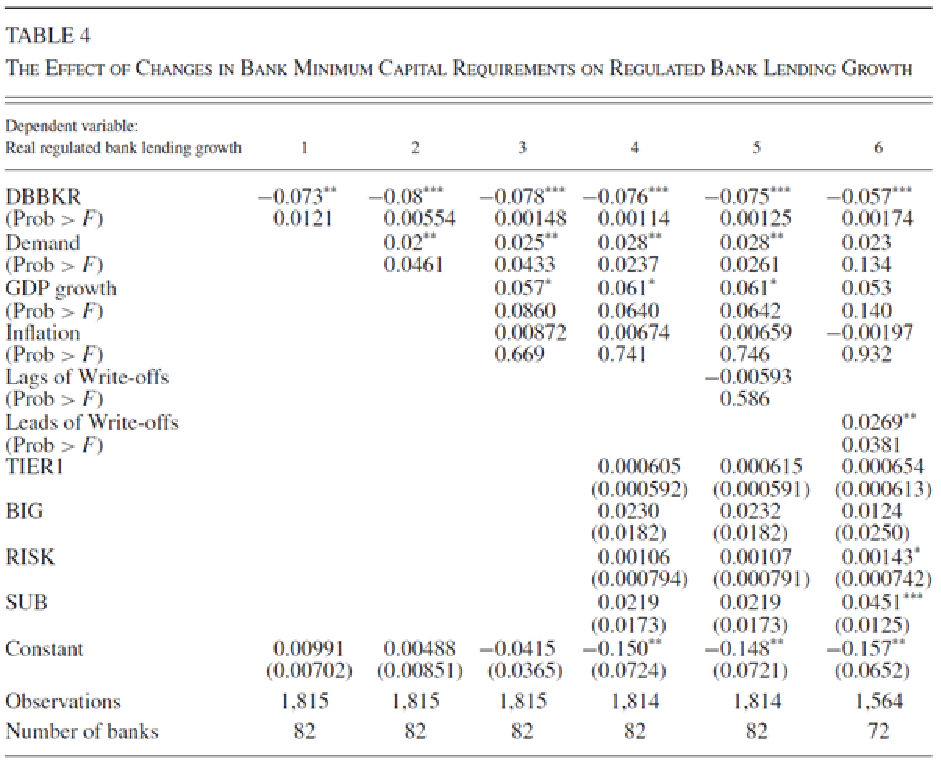
\includegraphics[width=\textwidth, height = 8cm]{AiyarEtAl_JMCB_2014_Table4}
\end{frame}

\begin{frame}{Fang \emph{et al.} (2020)}
\protect\hypertarget{fang2020bank}{}
\centering

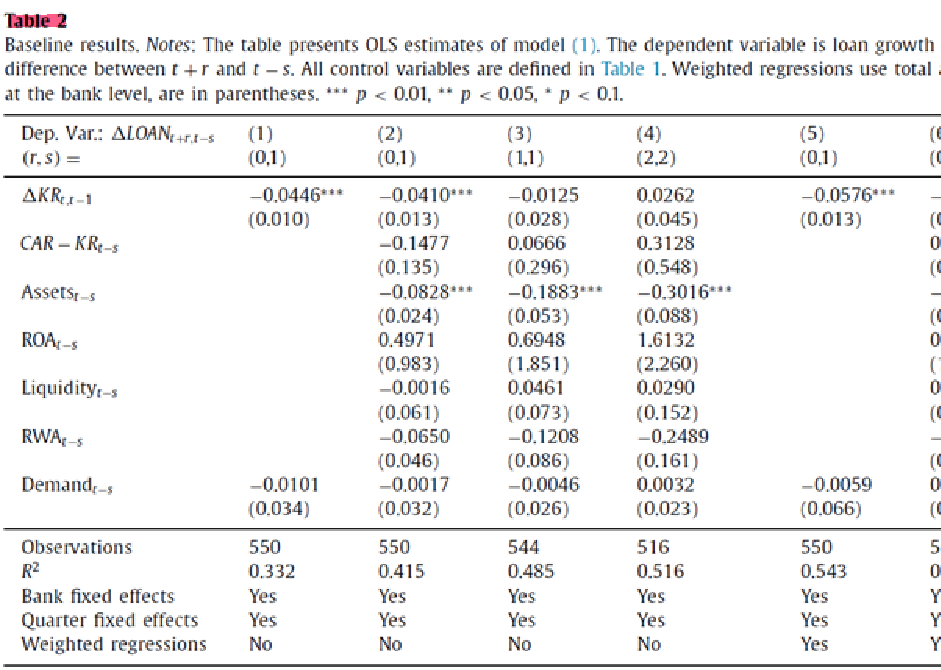
\includegraphics[width=\textwidth, height = 8cm]{FamgEtAl_JBF_2022}
\end{frame}

\begin{frame}{Some reasons to be cautious}
\protect\hypertarget{some-reasons-to-be-cautious}{}
\begin{itemize}
    \item theoretical prior, changes in required bank capital RBC impact lending 
    \begin{itemize}
        \item in SR, but not LR
        \item only marginally, even in SR, when
        \begin{enumerate}
            \item banks are fully capitalised OR
            \item capital increase is flagged well in advance
        \end{enumerate}
    \end{itemize}
    \item Demand variable does not fully address endogeneity
    \begin{itemize}
        \item Aiyar at al, Minimum capital $\uparrow$, a response to unsustainable lending
        \item Fang et al, seasonal reallocation of credit
    \end{itemize}
\end{itemize}
\end{frame}

\begin{frame}{Seasonal reallocation of credit}
\protect\hypertarget{seasonal-reallocation-of-credit}{}
\begin{itemize}
\item Composition bank credit across banks varies seasonally  
\begin{itemize}
    \item examples: Xmas, agricultural seasons
\end{itemize}
\item May be a bigger concern when 
\begin{itemize}
    \item Interventions are seasonal, as they are for Basel III 
    \item Bank customer base varies 
    \item Focusing on relative growth of bank credit (i.e. including time dummies)
\end{itemize}
\item Corrections?
\begin{itemize}
    \item Not corrected by standard demand proxy  
    \item Statistically impact should reduce using disaggregated loan categories  
    \item Or possibly correcting for demand using loan margins data
\end{itemize}
\end{itemize}
\end{frame}

\begin{frame}{SA banking sector}
\protect\hypertarget{sa-banking-sector}{}
\begin{itemize}
\tightlist
\item
  There are 34 active licensed banks in South Africa
\item
  As of April, 2020, the \% of banking sector assets: Standard Bank of
  South Africa (24.1\%), First Rand (20.4\%), ABSA (19.8\%), Nedbank
  (17.0\%) and Investec (7.8\%); the next largest bank is Capitec (2\%)
\item
  The ratio of bank assets to GDP is 112\%
\item
  This prudential regulation and South Africa's well-capitalised banking
  sector has prevented the emergence any systemic financial crisis
\end{itemize}
\end{frame}

\begin{frame}{Basel III capital framework}
\protect\hypertarget{basel-iii-capital-framework}{}
\begin{table}
\centering\begingroup\fontsize{10}{12}\selectfont

\begin{tabular}{>{\raggedright\arraybackslash}p{10cm}l}
\toprule
\multicolumn{2}{c}{Basel III capital requirement structure} \\
\cmidrule(l{3pt}r{3pt}){1-2}
Category & Percent\\
\midrule
Basel III minima & 8\\
South African minima & 8\\
Pillar 2A & 0.5 to 2\\
South Africa base minima & 8 + Pillar 2A\\
Pillar 2B (ICR) & no specific range\\
\addlinespace
Prudential minima & 8 + Pillar2A + ICR\\
Systemically important buffer & 0.5 to 2.5\\
Capital conservation buffer & 0 to 2.5\\
Countercyclical buffer & 0 to 2.5\\
\bottomrule
\end{tabular}
\endgroup{}
\end{table}
\end{frame}

\begin{frame}{Incremental implementation of capital requirments}
\protect\hypertarget{incremental-implementation-of-capital-requirments}{}
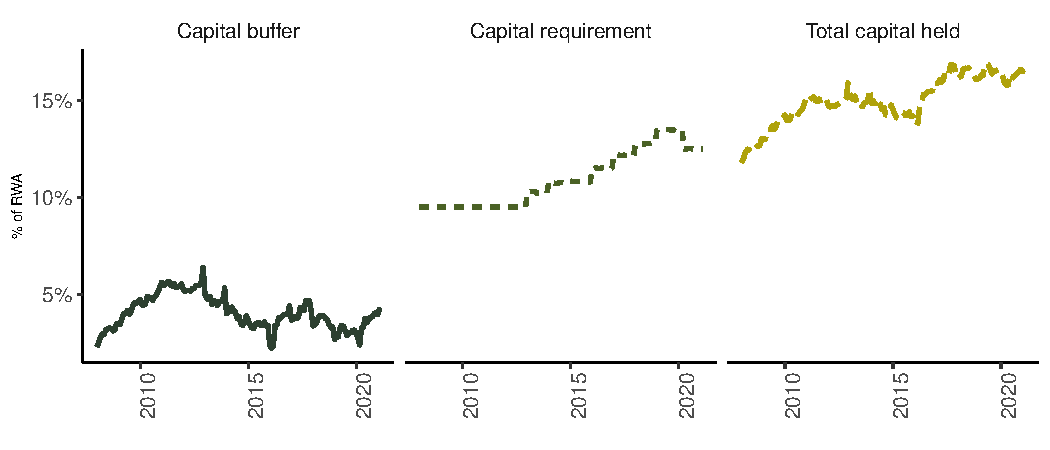
\includegraphics{baseIII_and_bank_lending_files/figure-beamer/capital-1.pdf}
\end{frame}

\begin{frame}{Data}
\protect\hypertarget{data}{}
\begin{itemize}
\tightlist
\item
  We collected data on the four major South African banks: Absa Bank,
  Standard Bank, First National Bank, and Nedbank
\item
  Mainly utilised the BA900s (bank economic returns) and the BA930s
  (bank product lending rates)
\item
  The Basel III capital requirements (BA700s) data was collected from
  the Prudential Authority
\item
  From the Prudential Authority, we also collected the controls data
\item
  We focus on real economic activity lending in the BA900s is
  represented by lending to households and non-financial corporations.
\item
  However, the BA900s only report granular lending categories to
  households and non-financial corporations. Therefore, some aggregation
  was necessary.
\item
  This aggregation essentially limited our sample to the big four
  lenders
\item
  Three major categories for households and non financial corporations
  (secured, unsecured, and mortgages)
\end{itemize}
\end{frame}

\begin{frame}{Methodology}
\protect\hypertarget{methodology}{}
Building on Fang \emph{et al.} (2020):

\(\Delta LOAN^i_{t, t-s} = \beta \Delta KR^i_{t, t-1} + \lambda \Delta KS^i_{t, t-1} + \alpha \Delta Demand^i_{t, t-1} + \gamma' \pmb{X}^i_{t-s} + \phi^i + \tau_t + \varepsilon^i_t.\)

\begin{itemize}
\tightlist
\item
  \(^i\) refers to the four banks
\item
  \(\Delta LOAN^i_{t, t-s}\) is the log difference of lending
\item
  \(\Delta KR^i_{t, t-1}\) is the change in the minimum capital
  requirement
\item
  \(\Delta Demand^i_{t, t-1}\) is the lending demand proxy represented
\item
  \(\pmb{X}^i_{t-s}\) is a bank level controls set at month \(t-s\).
\item
  The fixed effects (\(\phi^i\)) estimate other unobserved differences
  in bank characteristics.
\item
  To account for other factors, such as changes in the macroeconomic
  environment, we employ time-fixed effects (\(\tau_t\)).
\item
  \(\varepsilon^i_t\) using bank clustered standard errors
\end{itemize}
\end{frame}

\begin{frame}{Identification}
\protect\hypertarget{identification}{}
\begin{itemize}
\tightlist
\item
  However, there are challenges with the identification of
  \(\Delta KR^i_{t, t-1}\) (Fang \emph{et al.}, 2020)
\item
  That is, it is not just the changes due to Basel III that are included
  in \(\Delta KR^i_{t, t-1}\)
\item
  We isolate the Basel III related changes using a dummy structure (1
  when there are Basel III related changes, and 0 otherwise)
\item
  This ensures that we are estimating the Basel III impact and not other
  balance sheet related adjustments
\item
  Furthermore, we use a novel approach in estimating
  \(\Delta Demand^i_{t, t-1}\) as compared to Fang \emph{et al.} (2020)
  and others. However, most studies found demand effects tend to be
  insignificant
\end{itemize}
\end{frame}

\begin{frame}{Results I}
\protect\hypertarget{results-i}{}
\begin{table}
\centering\begingroup\fontsize{10}{12}\selectfont

\resizebox{\linewidth}{!}{
\begin{tabular}{>{\raggedright\arraybackslash}p{7cm}lllll}
\toprule
\multicolumn{6}{c}{Household secured credit} \\
\cmidrule(l{3pt}r{3pt}){1-6}
  & (1) & (2) & (3) & (4) & (5)\\
\midrule
$\Delta KR_{t,t-1}$ & -0.0060*** & -0.0062*** & -0.0036** & -0.0060*** & -0.0031\\
 & (0.0016) & (0.0014) & (0.0017) & (0.0016) & (0.0022)\\
$\Delta KS_{t,t-1}$ &  & -0.0966 & -0.0434 & -0.0603 & -0.0062\\
 &  & (0.1297) & (0.1585) & (0.1109) & (0.1161)\\
$\Delta Demand_{t,t-1}$ &  &  & 0.0038 &  & 0.0035\\
\addlinespace
 &  &  & (0.0037) &  & (0.0048)\\
$ROA_{t-1}$ &  &  &  & 0.3250 & 0.2359\\
 &  &  &  & (1.1751) & (1.3343)\\
$ROE_{t-1}$ &  &  &  & -0.0936 & -0.0848\\
 &  &  &  & (0.0987) & (0.1101)\\
\addlinespace
$Liquidity_{t-1}$ &  &  &  & -0.0076 & -0.0077\\
 &  &  &  & (0.0074) & (0.0081)\\
Num.Obs. & 372 & 372 & 369 & 368 & 365\\
Test of equality (p-value) & 0.00 & 0.00 & 0.08 & 0.00 & 0.30\\
Adj.R squared & 0.29 & 0.29 & 0.29 & 0.32 & 0.31\\
\bottomrule
\multicolumn{6}{l}{\rule{0pt}{1em}\textit{Note: }}\\
\multicolumn{6}{l}{\rule{0pt}{1em}The dependant variables in loan growth at bank level at a monthly frequency, calculated as the log difference at t and t -1.}\\
\multicolumn{6}{l}{\rule{0pt}{1em}Standard errors are clustered at a bank level.}\\
\multicolumn{6}{l}{\rule{0pt}{1em}All equations include both bank and monthly effects. A test for equality p-value of < 0.1 is significant.}\\
\multicolumn{6}{l}{\rule{0pt}{1em}*** p < 0.01, ** p < 0.05, * p < 0.1)}\\
\end{tabular}}
\endgroup{}
\end{table}
\end{frame}

\begin{frame}{Results II}
\protect\hypertarget{results-ii}{}
\begin{table}
\centering\begingroup\fontsize{10}{12}\selectfont

\resizebox{\linewidth}{!}{
\begin{tabular}{>{\raggedright\arraybackslash}p{7cm}lllll}
\toprule
\multicolumn{6}{c}{Household unsecured credit} \\
\cmidrule(l{3pt}r{3pt}){1-6}
  & (1) & (2) & (3) & (4) & (5)\\
\midrule
$\Delta KR_{t,t-1}$ & -0.0081*** & -0.0087*** & -0.0025 & -0.0084*** & -0.0017\\
 & (0.0017) & (0.0022) & (0.0029) & (0.0017) & (0.0030)\\
$\Delta KS_{t,t-1}$ &  & -0.2809 & -0.1138 & -0.2405 & -0.0762\\
 &  & (0.1841) & (0.1996) & (0.1619) & (0.1696)\\
$\Delta Demand_{t,t-1}$ &  &  & -0.0035 &  & -0.0042\\
\addlinespace
 &  &  & (0.0032) &  & (0.0032)\\
$ROA_{t-1}$ &  &  &  & 1.0548 & 0.7079\\
 &  &  &  & (1.2607) & (1.1998)\\
$ROE_{t-1}$ &  &  &  & -0.0920 & -0.0731\\
 &  &  &  & (0.1030) & (0.1015)\\
\addlinespace
$Liquidity_{t-1}$ &  &  &  & -0.0039 & -0.0012\\
 &  &  &  & (0.0071) & (0.0070)\\
Num.Obs. & 372 & 372 & 368 & 368 & 364\\
Test of equality (p-value) & 0.00 & 0.00 & 0.08 & 0.00 & 0.83\\
Adj.R squared & 0.38 & 0.39 & 0.39 & 0.36 & 0.37\\
\bottomrule
\multicolumn{6}{l}{\rule{0pt}{1em}\textit{Note: }}\\
\multicolumn{6}{l}{\rule{0pt}{1em}The dependant variables in loan growth at bank level at a monthly frequency, calculated as the log difference at t and t -1.}\\
\multicolumn{6}{l}{\rule{0pt}{1em}Standard errors are clustered at a bank level.}\\
\multicolumn{6}{l}{\rule{0pt}{1em}All equations include both bank and monthly effects. A test for equality p-value of < 0.1 is significant.}\\
\multicolumn{6}{l}{\rule{0pt}{1em}*** p < 0.01, ** p < 0.05, * p < 0.1)}\\
\end{tabular}}
\endgroup{}
\end{table}
\end{frame}

\begin{frame}{Results III}
\protect\hypertarget{results-iii}{}
\begin{table}
\centering\begingroup\fontsize{10}{12}\selectfont

\resizebox{\linewidth}{!}{
\begin{tabular}{>{\raggedright\arraybackslash}p{7cm}lllll}
\toprule
\multicolumn{6}{c}{Household mortgages} \\
\cmidrule(l{3pt}r{3pt}){1-6}
  & (1) & (2) & (3) & (4) & (5)\\
\midrule
$\Delta KR_{t,t-1}$ & -0.0023*** & -0.0023*** & -0.0023*** & -0.0026*** & -0.0026***\\
 & (0.0005) & (0.0004) & (0.0004) & (0.0004) & (0.0004)\\
$\Delta KS_{t,t-1}$ &  & -0.0193 & -0.0186 & -0.0057 & -0.0046\\
 &  & (0.0153) & (0.0161) & (0.0159) & (0.0160)\\
$\Delta Demand_{t,t-1}$ &  &  & 0.0001 &  & 0.0000\\
\addlinespace
 &  &  & (0.0011) &  & (0.0009)\\
$ROA_{t-1}$ &  &  &  & 0.4725* & 0.4959*\\
 &  &  &  & (0.2692) & (0.2719)\\
$ROE_{t-1}$ &  &  &  & -0.0396** & -0.0410**\\
 &  &  &  & (0.0176) & (0.0170)\\
\addlinespace
$Liquidity_{t-1}$ &  &  &  & 0.0026 & 0.0026\\
 &  &  &  & (0.0021) & (0.0022)\\
Num.Obs. & 372 & 372 & 368 & 368 & 364\\
Test of equality (p-value) & 0.00 & 0.00 & 0.00 & 0.00 & 0.00\\
Adj.R squared & 0.59 & 0.59 & 0.59 & 0.63 & 0.63\\
\bottomrule
\multicolumn{6}{l}{\rule{0pt}{1em}\textit{Note: }}\\
\multicolumn{6}{l}{\rule{0pt}{1em}The dependant variables in loan growth at bank level at a monthly frequency, calculated as the log difference at t and t -1.}\\
\multicolumn{6}{l}{\rule{0pt}{1em}Standard errors are clustered at a bank level.}\\
\multicolumn{6}{l}{\rule{0pt}{1em}All equations include both bank and monthly effects. A test for equality p-value of < 0.1 is significant.}\\
\multicolumn{6}{l}{\rule{0pt}{1em}*** p < 0.01, ** p < 0.05, * p < 0.1)}\\
\end{tabular}}
\endgroup{}
\end{table}
\end{frame}

\begin{frame}{Results IV}
\protect\hypertarget{results-iv}{}
\begin{table}
\centering\begingroup\fontsize{10}{12}\selectfont

\resizebox{\linewidth}{!}{
\begin{tabular}{>{\raggedright\arraybackslash}p{7cm}lllll}
\toprule
\multicolumn{6}{c}{Non financial corporations secured credit} \\
\cmidrule(l{3pt}r{3pt}){1-6}
  & (1) & (2) & (3) & (4) & (5)\\
\midrule
$\Delta KR_{t,t-1}$ & -0.0100*** & -0.0102*** & -0.0048* & -0.0096*** & -0.0052**\\
 & (0.0018) & (0.0019) & (0.0027) & (0.0021) & (0.0025)\\
$\Delta KS_{t,t-1}$ &  & -0.0845 & 0.0538 & -0.0145 & 0.0893\\
 &  & (0.1095) & (0.1031) & (0.1126) & (0.1223)\\
$\Delta Demand_{t,t-1}$ &  &  & 0.0040* &  & 0.0106***\\
\addlinespace
 &  &  & (0.0023) &  & (0.0022)\\
$ROA_{t-1}$ &  &  &  & 0.3812 & 0.4672\\
 &  &  &  & (1.1936) & (1.1979)\\
$ROE_{t-1}$ &  &  &  & -0.0559 & -0.0574\\
 &  &  &  & (0.0700) & (0.0688)\\
\addlinespace
$Liquidity_{t-1}$ &  &  &  & -0.0160*** & -0.0176***\\
 &  &  &  & (0.0027) & (0.0026)\\
Num.Obs. & 372 & 372 & 368 & 368 & 364\\
Test of equality (p-value) & 0.00 & 0.00 & 0.03 & 0.00 & 0.00\\
Adj.R squared & 0.25 & 0.25 & 0.25 & 0.28 & 0.28\\
\bottomrule
\multicolumn{6}{l}{\rule{0pt}{1em}\textit{Note: }}\\
\multicolumn{6}{l}{\rule{0pt}{1em}The dependant variables in loan growth at bank level at a monthly frequency, calculated as the log difference at t and t -1.}\\
\multicolumn{6}{l}{\rule{0pt}{1em}Standard errors are clustered at a bank level.}\\
\multicolumn{6}{l}{\rule{0pt}{1em}All equations include both bank and monthly effects. A test for equality p-value of < 0.1 is significant.}\\
\multicolumn{6}{l}{\rule{0pt}{1em}*** p < 0.01, ** p < 0.05, * p < 0.1)}\\
\end{tabular}}
\endgroup{}
\end{table}
\end{frame}

\begin{frame}{Results V}
\protect\hypertarget{results-v}{}
\begin{table}
\centering\begingroup\fontsize{10}{12}\selectfont

\resizebox{\linewidth}{!}{
\begin{tabular}{>{\raggedright\arraybackslash}p{7cm}lllll}
\toprule
\multicolumn{6}{c}{Non financial corporations unsecured credit} \\
\cmidrule(l{3pt}r{3pt}){1-6}
  & (1) & (2) & (3) & (4) & (5)\\
\midrule
$\Delta KR_{t,t-1}$ & 0.0034 & 0.0027 & 0.0020 & 0.0067 & 0.0025\\
 & (0.0085) & (0.0088) & (0.0082) & (0.0112) & (0.0096)\\
$\Delta KS_{t,t-1}$ &  & -0.3137 & -0.3602 & 0.0630 & -0.0476\\
 &  & (0.6473) & (0.7107) & (0.6036) & (0.6553)\\
$\Delta Demand_{t,t-1}$ &  &  & 0.0083* &  & 0.0168***\\
\addlinespace
 &  &  & (0.0046) &  & (0.0050)\\
$ROA_{t-1}$ &  &  &  & 4.3277*** & 4.5384***\\
 &  &  &  & (1.4400) & (1.2892)\\
$ROE_{t-1}$ &  &  &  & -0.2063*** & -0.2165**\\
 &  &  &  & (0.0655) & (0.0845)\\
\addlinespace
$Liquidity_{t-1}$ &  &  &  & -0.0331*** & -0.0384***\\
 &  &  &  & (0.0097) & (0.0091)\\
Num.Obs. & 372 & 372 & 364 & 368 & 360\\
Test of equality (p-value) & 0.69 & 0.64 & 0.33 & 0.81 & 0.92\\
Adj.R squared & 0.10 & 0.10 & 0.11 & 0.15 & 0.16\\
\bottomrule
\multicolumn{6}{l}{\rule{0pt}{1em}\textit{Note: }}\\
\multicolumn{6}{l}{\rule{0pt}{1em}The dependant variables in loan growth at bank level at a monthly frequency, calculated as the log difference at t and t -1.}\\
\multicolumn{6}{l}{\rule{0pt}{1em}Standard errors are clustered at a bank level.}\\
\multicolumn{6}{l}{\rule{0pt}{1em}All equations include both bank and monthly effects. A test for equality p-value of < 0.1 is significant.}\\
\multicolumn{6}{l}{\rule{0pt}{1em}*** p < 0.01, ** p < 0.05, * p < 0.1)}\\
\end{tabular}}
\endgroup{}
\end{table}
\end{frame}

\begin{frame}{Results VI}
\protect\hypertarget{results-vi}{}
\begin{table}
\centering\begingroup\fontsize{10}{12}\selectfont

\resizebox{\linewidth}{!}{
\begin{tabular}{>{\raggedright\arraybackslash}p{7cm}lllll}
\toprule
\multicolumn{6}{c}{Non financial corporations mortgage credit} \\
\cmidrule(l{3pt}r{3pt}){1-6}
  & (1) & (2) & (3) & (4) & (5)\\
\midrule
$\Delta KR_{t,t-1}$ & 0.0022 & 0.0014 & 0.0022 & 0.0005 & 0.0015\\
 & (0.0026) & (0.0027) & (0.0027) & (0.0027) & (0.0032)\\
$\Delta KS_{t,t-1}$ &  & -0.3535** & -0.3415** & -0.4139*** & -0.4030***\\
 &  & (0.1407) & (0.1398) & (0.1359) & (0.1434)\\
$\Delta Demand_{t,t-1}$ &  &  & -0.0050*** &  & -0.0055***\\
\addlinespace
 &  &  & (0.0014) &  & (0.0009)\\
$ROA_{t-1}$ &  &  &  & 1.4596 & 1.2758\\
 &  &  &  & (2.0032) & (2.1460)\\
$ROE_{t-1}$ &  &  &  & -0.0947 & -0.0819\\
 &  &  &  & (0.1459) & (0.1428)\\
\addlinespace
$Liquidity_{t-1}$ &  &  &  & 0.0075 & 0.0081\\
 &  &  &  & (0.0063) & (0.0088)\\
Num.Obs. & 372 & 372 & 368 & 368 & 364\\
Test of equality (p-value) & 0.43 & 0.00 & 0.00 & 0.00 & 0.00\\
Adj.R squared & 0.12 & 0.13 & 0.13 & 0.14 & 0.14\\
\bottomrule
\multicolumn{6}{l}{\rule{0pt}{1em}\textit{Note: }}\\
\multicolumn{6}{l}{\rule{0pt}{1em}The dependant variables in loan growth at bank level at a monthly frequency, calculated as the log difference at t and t -1.}\\
\multicolumn{6}{l}{\rule{0pt}{1em}Standard errors are clustered at a bank level.}\\
\multicolumn{6}{l}{\rule{0pt}{1em}All equations include both bank and monthly effects. A test for equality p-value of < 0.1 is significant.}\\
\multicolumn{6}{l}{\rule{0pt}{1em}*** p < 0.01, ** p < 0.05, * p < 0.1)}\\
\end{tabular}}
\endgroup{}
\end{table}
\end{frame}

\begin{frame}{Timevarying estimates via local projections (Jordà, 2005)}
\protect\hypertarget{timevarying-estimates-via-local-projections-jorda2005estimation}{}
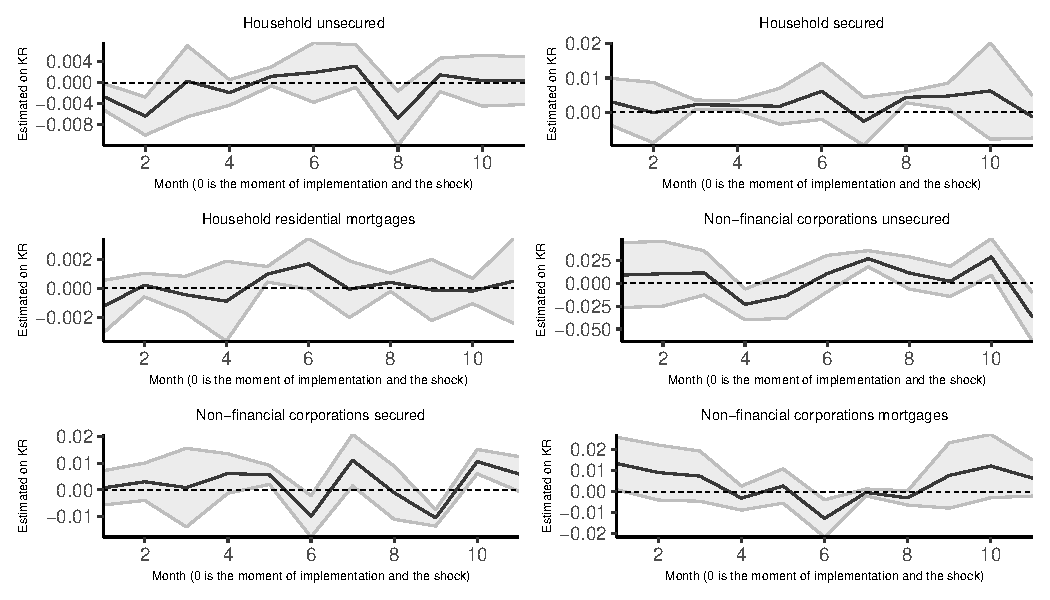
\includegraphics{baseIII_and_bank_lending_files/figure-beamer/path-1.pdf}
\end{frame}

\begin{frame}{Conclusion I}
\protect\hypertarget{conclusion-i}{}
\begin{itemize}
\tightlist
\item
  Our estimates of between 0.48 and 2.4 percentage points are lower than
  Fang \emph{et al.} (2020) estimates of 4 to 6 percentage points
\item
  However, they are closer to the UK, where Aiyar, Calomiris and
  Wieladek (2016) found 0.55 percentage points
\item
  The SARB's gradual approach resulted in a comparably lower lending
  effect
\item
  Although they focus on the impact of the surplus capital buffer on
  lending in South Africa, in their estimations Pillay and Makrelov
  (2023) similar magnitudes on the impact of capital requirements on
  lending.
\item
  The lower estimates are not surprising as the extent of the reduction
  in lending primarily depends on how expensive it is for banks to raise
  equity (Aiyar, Calomiris and Wieladek, 2016). South African banks, in
  addition, to the capital requirements, kept a significant capital
  buffer.
\end{itemize}
\end{frame}

\begin{frame}{Conclusion II}
\protect\hypertarget{conclusion-ii}{}
\begin{itemize}
\tightlist
\item
  The results also revealed a more significant effect on household
  lending versus non-financial corporation lending.
\item
  One explanation is that it is much easier for banks to discriminate
  between borrowers in their commercial business versus retail business
  when banks need to reduce their risk-weighted assets to meet higher
  capital requirements (De Jonghe, Dewachter and Ongena, 2020).
\item
  There are fewer clients on the commercial side, and the assets are
  larger. This higher asset base also suggests that banks are more
  careful or place more risk-weights on lending on the commercial than
  the household side (Imbierowicz, Kragh and Rangvid, 2018).
\item
  In South Africa, this means that banks avoid having to pull back on
  lending on the commercial side as a result of higher capital
  requirements, with the capital buffer as a first `shock-absorber'.
\item
  The issue of demand effect remains a concern
\item
  Further capital requirement endogeneity is possible in the form of
  anticipation effects. We attempt to address these in the paper.
\end{itemize}
\end{frame}

\begin{frame}{Thank You!}
\protect\hypertarget{thank-you}{}
\centering Thank You!
\end{frame}

\begin{frame}[allowframebreaks]{References}
\protect\hypertarget{references}{}
\hypertarget{refs}{}
\begin{CSLReferences}{0}{0}
\leavevmode\vadjust pre{\hypertarget{ref-aiyar2014international}{}}%
Aiyar, S., Calomiris, C. W., Hooley, J., Korniyenko, Y. and Wieladek, T.
(2014). {`The international transmission of bank capital requirements:
Evidence from the UK'}. \emph{Journal of Financial Economics}. Elsevier,
113 (3), pp. 368--382.

\leavevmode\vadjust pre{\hypertarget{ref-aiyar2016does}{}}%
Aiyar, S., Calomiris, C. W. and Wieladek, T. (2016). {`How does credit
supply respond to monetary policy and bank minimum capital
requirements?'} \emph{European Economic Review}. Elsevier, 82, pp.
142--165.

\leavevmode\vadjust pre{\hypertarget{ref-berger1994lines}{}}%
Berger, A. N. and Udell, G. F. (1994). {`Lines of credit and
relationship lending in small firm finance'}. \emph{Jerome Levy
Economics Institute Working Paper}, (113).

\leavevmode\vadjust pre{\hypertarget{ref-de2020bank}{}}%
De Jonghe, O., Dewachter, H. and Ongena, S. (2020). {`Bank capital
(requirements) and credit supply: Evidence from pillar 2 decisions'}.
\emph{Journal of Corporate Finance}. Elsevier, 60, p. 101518.

\leavevmode\vadjust pre{\hypertarget{ref-fang2020bank}{}}%
Fang, X., Jutrsa, D., Peria, S. M., Presbitero, A. F. and Ratnovski, L.
(2020). {`Bank capital requirements and lending in emerging markets: The
role of bank characteristics and economic conditions'}. \emph{Journal of
Banking \& Finance}. Elsevier, p. 105806.

\leavevmode\vadjust pre{\hypertarget{ref-francis2012capital}{}}%
Francis, W. B. and Osborne, M. (2012). {`Capital requirements and bank
behavior in the UK: Are there lessons for international capital
standards?'} \emph{Journal of Banking \& Finance}. Elsevier, 36 (3), pp.
803--816.

\leavevmode\vadjust pre{\hypertarget{ref-houston1997capital}{}}%
Houston, J., James, C. and Marcus, D. (1997). {`Capital market frictions
and the role of internal capital markets in banking'}. \emph{Journal of
financial Economics}. Elsevier, 46 (2), pp. 135--164.

\leavevmode\vadjust pre{\hypertarget{ref-imbierowicz2018time}{}}%
Imbierowicz, B., Kragh, J. and Rangvid, J. (2018). {`Time-varying
capital requirements and disclosure rules: Effects on capitalization and
lending decisions'}. \emph{Journal of Money, Credit and Banking}. Wiley
Online Library, 50 (4), pp. 573--602.

\leavevmode\vadjust pre{\hypertarget{ref-jorda2005estimation}{}}%
Jordà, Ò. (2005). {`Estimation and inference of impulse responses by
local projections'}. \emph{American economic review}. American Economic
Association, 95 (1), pp. 161--182.

\leavevmode\vadjust pre{\hypertarget{ref-nier2005bank}{}}%
Nier, E. and Zicchino, L. (2005). {`Bank weakness and bank loan
supply'}. \emph{Bank of England Financial Stability Review (December)},
pp. 85--93.

\leavevmode\vadjust pre{\hypertarget{ref-peek1997international}{}}%
Peek, J. and Rosengren, E. S. (1997). {`The international transmission
of financial shocks: The case of japan'}. \emph{The American Economic
Review}. JSTOR, pp. 495--505.

\leavevmode\vadjust pre{\hypertarget{ref-neryvia2023}{}}%
Pillay, N. and Makrelov, K. (2023). {`Capital buffers and lending in
south africa (upcoming)'}. South African Reserve Bank.

\leavevmode\vadjust pre{\hypertarget{ref-van2008welfare}{}}%
Van den Heuvel, S. J. (2008). {`The welfare cost of bank capital
requirements'}. \emph{Journal of Monetary Economics}. Elsevier, 55 (2),
pp. 298--320.

\end{CSLReferences}
\end{frame}

\end{document}
